\label{theproblem}

A signalized intersection, or network of intersections, has a number of key parameters, which are essential to the performance of the intersection.

\begin{description}
\item[Cycle time] is the time from a sequence of phases begins until they are looped again. The cycle time is very important to the chosen MOE. In \cite{41} Sun et al. explain that 

\begin{quote}[...] minimizing delay leads to short cycle length while minimizing stops indicates long cycle length.
\end{quote}

The reason is that a long cycle length may stop many vehicles in a platoon and incur a large delay for them, but the platoon of vehicles only experience a single stop. With short cycle time the vehicles never have to wait long for a green light but are more stopped more frequently in average.

Most authors who consider coordination of multiple signals use and optimize a cycle time which is common for all traffic signals since it would otherwise become hard to coordinate signals in static schedules. In a small network, if each signal operates on its own cycle time, green waves would only work on a periodic basis when the cycle time and offset parameters of all signals eclipse otherwise the green wave would drift and either cut off platoons of vehicles or give too much green time.

The cycle time of an intersection is one of the most important parameters in a signal plan since it sets  lower and upper bounds on the green times for the phases. This relates to the MOE as well as the safety of a network since 1) if a red light is shown for too long some trafficants may start to ignore the signals and 2) if the signals cycle too frequently there is an increased risk of collisions.

\item[Green split]  is the proportion of cycle time which is to be green in one direction and red in the opposing directions. 

The green split should be considered as an indication of the amount of traffic expected from each road facing the intersection. Major roads will be given the larger split and minor roads a smaller split.

\item[Offset] is the amount of time, relative to the common cycle time, for which an intersection should starts it's sequence. The offset for an intersection is used to accomodate green waves for traffic travelling from intersection to intersection at a specified pace.

This parameter is mostly relevant when optimizing signal plans for major-minor types of arterials where platoons travel (mostly) along a path which traverse a string of intersections. Some of the most promising results for this specific type of optimization are from MAXBAND and MULTIBAND, described in \cite{37}.

\end{description}

Almost all methods optimize some or all of these parameters. A less commonly optimized parameter is the \textit{phase sequence} ie. the order in which phases should be green during a cycle. This is mostly relevant when prioritizing certain types traffic eg. public (see \cite{scoot2004}) or emergency vehicles but also when considering safety aspects.

The problem of choosing a MOE is subtle in its own and depends on eg:

\begin{itemize}
\item The type of traffic which should gain benefits: private and commercial vehicles, public transportation, soft trafficants ie. pedestrians and bicyclists
\item The network: highway, rural, urban
\item Political objectives: safety, priority to businesses, reduction of emmisions (combined with more public transportation and \textit{green} buses
\end{itemize}

Clearly there are conflicts of interest among this selection of objectives. Some examples have already been mentioned, additional examples of objective conflicts are:

\begin{itemize}
\item Minimizing delays for vehicles along an artery will cause longer waiting times for crossing pedestrians
\item Prioritizing eg. public transport by skipping a phase will lower the performance for private transport. 

In the SCOOT system \cite{scoot2004} a phase skipping approach to bus prioritization was implemented and tested in a London intersection. The buses enjoyed 4$s$ less delay but the delay for non-bus vehicles increased by 1$s$ in total average. The vehicles on the roads with no bus traffic suffered up to 14$s$ delay on average, however.
\item Finally, any optimization which improves the experience of traversing the network by vehicle will probably cause more traffic and thus increase emissions
\end{itemize}

Most of the articles in the survey use the average delay as objective. The TRANSYT optimization package by Robertson (1969) uses the PI as explained in \cite{26}:

\begin{quote}
The performance index
is defined as the sum for all signal-controlled traffic streams of a
weighted linear combination of estimated delay and number
of stops per unit time and is used to measure the overall cost of
traffic congestion associated with the traffic control plan.
\end{quote}

Thus TRANSYT faces the multiobjectivity but the weights must be defined and maintained by the traffic engineers supervising the system. This is no trivial task and requires intimate knowledge of the network as well as the optimization package. The TRANSYT manual and Danish Road Directorate agree that the weights should be set so that 1 stop $\simeq$ 20 seconds delay.

In \cite{41} a true multiobjective optimization approach is tested. Sun et al. use a Non-dominated Sorting Genetic Algorithms (NSGA II) to find Pareto-optimal\footnote{No changes can be made which improves upon at least one objective while no objective values worsen} solutions for the minimization objectives \textit{average delay} and \textit{number of stops} per unit of time. 

\subsection{Mathematical Model}
\label{model}
The problem is now formulated as the minimization of a selected performance index (PI) in terms of a set of signal settings, $\Psi$, and a network, which is dependent on the signal settings.

$$\min PI \left(  \Psi, N\left( \Psi\right)  \right)  $$

In a general, discrete time, model time each time steps are denoted by $t$. The network consists of $N \geq 1$ signal controlled intersections indexed by $n$.

In the model each signal is designated a phase for each time unit. Thus the concept of a cycle becomes virtual as they are no longer mandatory for calculating eg. the length of phases given the green splits.

Without a common cycle time - or individual cycle time, even - the offset parameter also disappears. However they can be made to exist virtually, in terms of a virtual cycle, and can thus be manipulated to excert the same behaviour. 
The main problem is during initialization when the system has just started. In this case it is possible synchronize intersections by delaying startup for those that would otherwise have a positive offset and vice versa for negative offset intersections. The same strategy can be used when increasing or decreasing the (virtual) cycle time for the arterial.

Phase sequences and green splits are unified by the specification of the phase in a timeslot, $t$, referred to as $p_n(t)$. For each intersection there will be a fixed number of phases, $P_n$, which are free from right-of-way conflicts. For a simple cross intersection with left-side driven vehicles (see figure \ref{fig:simple_intersection}) this number is 2: straight, left, and right turning flows in north and south directions for phase 1 and in east and west directions for phase 2.

\begin{figure}[!h]
\begin{center}
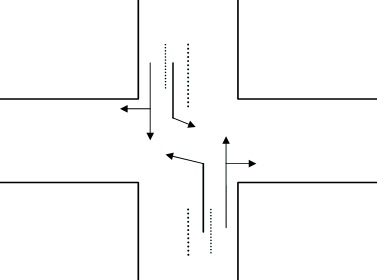
\includegraphics[scale=0.4]{simple_intersection.png} 
\end{center}
\label{fig:simple_intersection}
\caption{Simple intersection}
\end{figure}

Thus a specific phase $p = p_n(t) \in \lbrace 1,...,P_n \rbrace$ is selected for each timeslot. With this definition the green splits are implicit in the phase sequence. 

Now $\Psi = \lbrace \textbf{p} \rbrace $ and we can perform an optimization.

Satisfaction of minimum and maximum green times is the most common constraint, usually defined within a cycle. In this model the following equation must be satisfied:

$$
\forall p,n: \; T = \lbrace t: p_n(t) = p \rbrace \; st. \; cons(T) \wedge T_{min,p,n} \leq |T| \leq T_{max,p,n} 
$$
Thus $T$ is a set of points in time and the $cons$ function is defined by:
$$
cons(T) = 
\begin{cases}
true & if \;  \displaystyle\sum_{t \in T}{t} = � \cdot (\max T + \min T) \cdot (\max T - \min T + 1) \\
false & otherwise
\end{cases}
$$

That is, there must be a consecutive series of time slots (tested by using the Gaussian formula) in which phase $p$ is run.